\documentclass{article}

\usepackage[paper=letterpaper,margin=2.5cm]{geometry} % Set Margins

%% Math and math fonts
\usepackage{amsmath, amsthm, amssymb, amsfonts}
\usepackage{amsmath}
\usepackage{bbm} % for \mathbbm{1}

% date
\usepackage[nodayofweek]{datetime}

% Color
\usepackage{color, xcolor}

% Misc
\usepackage{environ}  % \collect@body in asmmath
\usepackage{graphicx} % \includegraphics options
\usepackage{mdframed} % text boxes
\usepackage{indentfirst} % Indent first paragraph after section header
\usepackage[shortlabels]{enumitem} % Control enumerate items with [(a)]
\usepackage{comment} % Comments
\usepackage{fancyhdr} % Headers and footers

% Tables
\usepackage{array}

% Sub-figures and figure placement
\usepackage{caption}
\usepackage{subcaption}
\usepackage{float} 

% Graphing
\usepackage{pgfplots}
\pgfplotsset{compat=1.17}
\usepackage{tikz}

% Title Placement
\usepackage{titling}
\setlength{\droptitle}{-6em}

%set indent to 
\setlength{\parindent}{0pt}

% Hyper refs
\usepackage{hyperref}
\hypersetup{
    colorlinks=true,
    linkcolor=blue,
    urlcolor  = blue,
    filecolor=magenta,      
    urlcolor=blue,
    citecolor = blue,
    anchorcolor = blue
}

% % Citation management
\usepackage{natbib}
\bibliographystyle{abbrvnat}
\setcitestyle{authordate,open={(},close={)}}

\pagestyle{fancy}

\usepackage[paper=letterpaper,margin=2.5cm]{geometry} % Set Margins

%% Math and math fonts
\usepackage{amsmath, amsthm, amssymb, amsfonts}
\usepackage{bbm} % for \mathbbm{1}

% date
\usepackage[nodayofweek]{datetime}

% Color
\usepackage{color, xcolor}

% Misc
\usepackage{environ}  % \collect@body in asmmath
\usepackage{graphicx} % \includegraphics options
\usepackage{mdframed} % text boxes
\usepackage{indentfirst} % Indent first paragraph after section header
\usepackage{comment} % Comments
\usepackage{fancyhdr} % Headers and footers

% Tables
\usepackage{array}

% Sub-figures and figure placement
\usepackage{caption}
% \usepackage{subcaption}
\usepackage{float} 

% Graphing
\usepackage{pgfplots}
\pgfplotsset{compat=1.17}
\usepackage{tikz}

% Title Placement
\usepackage{titling}
\setlength{\droptitle}{-6em}

%set indent to 
\setlength{\parindent}{0pt}

% Hyper refs
\usepackage{hyperref}
\hypersetup{
    colorlinks=true,
    linkcolor=blue,
    urlcolor  = blue,
    filecolor=magenta,      
    urlcolor=blue,
    citecolor = blue,
    anchorcolor = blue
}

% % Citation management
\usepackage{natbib}
\bibliographystyle{abbrvnat}
\setcitestyle{authordate,open={(},close={)}}

% ----------------------------------------
% TITLE
% ----------------------------------------

\pagestyle{fancy}

\lhead{Creel}
\chead{Probability and Integrals}
\rhead{AMES}

\title{AMES Class Notes -- Week 7, Monday: Integrals and Probability}
\author{Andie Creel}

\begin{document}
\maketitle

\section{Integration by parts}
Recall from Monday, integration by parts is an application of the product rule.  \\

Consider the function 
\begin{align}
    z(x) = f(x) g(x)
\end{align}

We want the integral of $z(x)$ 
\begin{align}
    Z(x) = \int f(x)g(x) dx 
\end{align}

Now, we know how to get $dz(x) /dx$ using the product rule
\begin{align}
    \frac{dz(x)}{dx} = f'(x) g(x) + f(x) g'(x) \implies\\
    \int dz = \int (f'(x) g(x) + f(x) g'(x)) dx 
\end{align}

Remember integrals are linear operators
\begin{align}
    \int dz = \int f'(x) g(x) dx + \int f(x) g'(x) dx\\
\end{align}
Note that $\int dz = z(x) = f(x) g(x)$
\begin{align}
    f(x) g(x) = \int f'(x) g(x) dx + \int f(x) g'(x) dx \implies \\
    f(x) g(x) - \int f(x) g'(x) dx = \int f'(x) g(x) dx \\
    f(x) g(x) - \int f(x) g'(x) dx = \int g(x) f'(x) dx  \\
    \int g(x) f'(x) dx = f(x) g(x) - \int f(x) g'(x) dx
\end{align}

Let 
\begin{align}
    U = g(x) \\
    dV = f'(x)dx \\
    V = f(x) \\
    dU = g'(x)dx
\end{align}
Plug these back into our last equation 

\begin{align}
    \int U dV = V U - \int V dU
\end{align}
which is the equation for integration by parts. \\


\section{Tips}
How can you remember the order of what should be U and what should be dV? \\
U $\rightarrow$ Log $\rightarrow$ Inverse trig $\rightarrow$ Algebraic $\rightarrow$ Trig $\rightarrow$ Exponential $\rightarrow$ dV \\


\section{Example}
Consider the function 
\begin{align}
    \int x  e^x dx
\end{align}

Whats's U and what's V? 
\begin{align}
    \int U dV = vu - \int V dU\\
    U = x\\
    dU = dx \\
    V = e^x\\
    dV = e^x dx
\end{align}

Rewrite the whole thing! And use integration by parts
\begin{align}
    \int x e^x dx &= e^x x - \int e^x dx \\
    &= x e^x - e^x \\
    &= (x - 1) e^x
\end{align}


\section{Integrating logs}

Consider the integral of $1/x$, which we know from knowing the derivative of $ln(x)$,
\begin{align}
    \int \frac{dx}{x} = \int \frac{1}{x} dx = ln(x)
\end{align}
Cool! Wait, but what the integral of a log,
\begin{align}
    \int ln(x) dx = ??
\end{align}
This was a really hard problem that existed for a very long time in mathematics. What's the trick? To use integration by parts, we consider this function instead 

\begin{align}
    \int ln(x) 1 dx 
\end{align}
Now we can use integration by parts and make the following variable assignments,

\begin{align}
    U = ln(x) \\
    dU = \frac{1}{x} dx\\
    V = x \\
    dV = 1 dx\\
\end{align}
\textbf{Do NOT forget the $dx$ when you get $dU$!!} Now, plug it all back into our integration by parts formal 
\begin{align}
    \int U dV &= V U - \int V dU\\
    \int ln(x) 1 dx &= x ln(x) - \int x \frac{1}{x} dx \implies \\
    &= x ln(x) - \int 1 dx  \\
    & = x ln(x) - x\\
    &= x (ln(x) - 1)
\end{align}
You can take the derivative of this final equation to check and you'll find the derivative of that final equation does equal $ln(x)$.

\section{Cross Partials Derivatives to Double Integrals}

We're going to take a \textbf{cross partial} derivative of a function (meaning derivative with respect to one variable and then derivative wrt a different variable). \\

We then are going to to do a \textbf{double integral} to reverse these two derivatives. \\

Consider the function 
\begin{align}
    F(x,y) = x^\alpha y^\beta \label{org}
\end{align}

Take the derivative with respect to $x$,
\begin{align}
    \frac{\partial F}{\partial x} = \alpha x^{\alpha -1}y ^\beta \label{derv}
\end{align}

Now, take the derivative of $\partial F / \partial x$ with respect to $y$, 
\begin{align}
    \frac{\partial F}{\partial x \partial y} = F_{x,y}(x,y) = \alpha \beta x^{\alpha -1} y^{\beta - 1}
\end{align}

Now, we can do a \textbf{double integral} to undo the two derivatives we've taken (cross partial). 

\begin{align}
    \int_x \int_y \alpha \beta x^{\alpha -1} y^{\beta - 1} dy dx
\end{align}
First, integrate with respect to y. To do so, we can pull the constants out front of the integral that has to do with variable $y$,
\begin{align}
   = \int_x \alpha \beta x^{\alpha -1}\int_y  y^{\beta - 1} dy dx\\
   = \int_x \alpha \frac{\beta}{\beta} x^{\alpha -1} y^\beta dx\\
   = \int_x \alpha x^{\alpha -1} y^\beta dx \label{int}
\end{align}

We have undone the derivative wrt to $y$ by integrating wrt $y$! Note that the term in the integral in equation \ref{int} is the same as \ref{derv}. We can now undo the integral wrt to $x$ by doing the integral wrt to $x$. 

\begin{align}
    = \frac{\alpha}{\alpha} x^\alpha y^\beta + C\\
    = x^\alpha y^\beta + C
\end{align}
and we have successfully returned to $F(x,y) = x^\alpha y^\beta +C$ which is the same as our original equation \ref{org} (plus an arbitrary constant).

\section{Double Integral}
We need to sum over one variable and then we sum over the other.
\begin{align}
    \int \int xy dx dy = \int \bigg(\int xy dx\bigg) dy 
\end{align}
We can solve the integral in parentheses first while treating $y$ like a constant 
\begin{align}
    &= \int \bigg( y\int x dx\bigg) dy \\
    &= \int \bigg( y\frac{1}{2} x^2 \bigg) dy
\end{align}
Now we can treat $x$ as a constant
\begin{align}
    &= \frac{1}{2} x^2 \int y dy\\
    & = \frac{1}{2} x^2 * \frac{1}{2} y^2 + C\\
    &= \frac{1}{4} x^2 y^2 + C
\end{align}

\section{Probability density function}

Consider the random variable $Y$. Random variables aren't random and they aren't variables. They're really more like functions. \\

\subsection{Normal Distribution}
If $Y$ is distributed normally it will look like 
\begin{align}
    Y = f(y) = \int_{- \infty}^{\infty} \frac{1}{\sigma \sqrt{2 \pi}} e^{-\frac{1}{2}(\frac{y - \mu}{\sigma})^2} dy = 1
\end{align}

the inside of the integral is the probability density function. The integral of a pdf must equal 1. 

% \subsection{Example}
% Consider the random variable 
% \begin{align}
%     Y = f(y) = 2y e^{-y^2}
% \end{align}

% and the support is $[0, \infty )$. Our probability density function (pdf) is $f(y)$. 

% Our cumulative distribution function (CDF) is 
% \begin{align}
%     CDF &= \int_0^\infty 2y e^{-y^2} dy \\
%     &= 2 \int_0^\infty y e^{-y^2} dy
% \end{align}

% Let $u = -y^2$, $du = -2y dy$
% \begin{align}
%     &= 2 \int_0^\infty  ye^u \frac{du}{-2y} \\
%     &= -1  \int_0^\infty e^u du \\
%     &= -1 e^u \bigg |_0^\infty \\
%     & = -1 e^{-y^2}\bigg |_0^\infty \\ 
%     & = 0 - - 1\\
%     & = 1
% \end{align}

% Which integrates to 1 after doing a u substitution, and so we know we have a proper pdf. \\

% What if you want to find the \textbf{median}? Set the CDF equal to $0.5$ because the median is the 50th percentile. \\

% The unknown is the point on the x-axis where the area under the pdf is equal to 0.5 (which is defined as our median). Start with equation 8 from our previous integral derivation because we know the integral is equal to that. But replace the upper bound to an unknown $\tilde{y}$ and set equal to 0.5.

% \begin{align}
%     -1 e^{-y^2} \bigg |_0^{\tilde {y}} &= 0.5\\
%     -e^{- \tilde y ^2} - - 1 &= 0. 5\\
%     -e^{- \tilde y ^2} &= - 0.5 \\  
%     e^{- \tilde y ^2} & = 0.5\\
%     ln( e^{- \tilde y ^2}) &= ln(1/2) \\
%     - \tilde y^2 &= ln(1/2)  \\
%     \tilde y^2 &= - ln(1/2) \\
%     \tilde y &= \sqrt{-ln(1/2)}
% \end{align}

% so we know that the median value is $\sqrt{- ln(1/2)}$.

% \begin{figure}[htp]
%     \centering
%         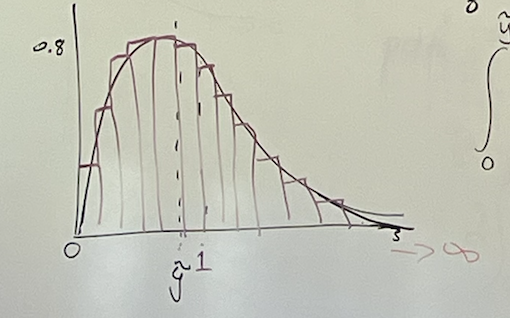
\includegraphics[width=0.5\textwidth]{Screen Shot 2023-10-09 at 11.11.30 AM.png}
%     \caption{Histograph}
%     % \label{fig:sample}
% \end{figure}

% \subsection{Mean}
% To find a mean, we sum the values and divide it by the number of people we summed over. This is the same as multiplying everyone's value by $\frac{1}{N}$. 
% \begin{align}
%    E[Y]= \bar y &= \frac{1}{N}\sum_n y_n\\
%    &= \sum_n \frac{1}{N} y_n
% \end{align}


% We can use the pdf to get our mean! The pdf would replace the $\frac{1}{N}$ and the sum would be replaced by the integral. 

% \begin{align}
%     E[Y]= \bar y = \int_0^\infty 2ye^{-y^2} * y dy
% \end{align}

% Important: I let the pdf be $f(y)$ for the mean and variance examples.
% \begin{align}
%     f(y) = pdf(y)
% \end{align}

% The general rule for finding the mean of a random variable by using the pdf $f(y)$ of that random variable is 
% \begin{align}
%     E[Y] = \int_\Omega y f(y) dy
% \end{align}
% where $\Omega$ is the support of $y$. \\

% \subsection{Function of the random variable}

% Now, let's say you're interest in the function of a mean. You're interested in $g(y)$ rather that $y$ itself.
% \begin{align}
%     E[g(y)] = \int_\Omega g(y) f(y) dy
% \end{align}
% where $f(y)$ continues to be the pdf of $Y$. This doesn't break jensen's inequality.

% \subsection{Variance}
% We an use the pdf to find the variance of $Y$, as well.
% \begin{align}
%         VAR(Y) = \int_\Omega y^2 f(y) dy - E(y)^2
% \end{align}

% \section{Uniform Distribution Example}
% Consider the uniform ditribution's pdf 
% \begin{align}
%     f(y) = \frac{1}{\theta_2 - \theta_1}
% \end{align}
% Let $\theta_2 = 1$ and $\theta_1 = 0$

% \begin{align}
%     f(y) = \frac{1}{1 - 0}\\
%     f(y) = 1
% \end{align}

% Prove $f(y)$ \textbf{is a pdf} by showing it integrates to 1. 
% \begin{align}
%     \int_0^1 1 dy = y \bigg|_0^1 = 1 - 0 = 1
% \end{align}

% What's the mean? 
% \begin{align}
%     E(Y) = \int_0^1 y *1 dy = \frac{1}{2} y^2 \bigg|_0^1 = \frac{1}{2}
% \end{align}

% What's the median? 
% \begin{align}
%     Med(Y) = \int_0^{\tilde y} dy = 0.5 \\
%     y\bigg|_0^{\tilde y} = 0.5 \\
%     \tilde y - 0 = 0.5
% \end{align}

% What's the variance?
% \begin{align}
%     Var(Y) &= \int_0^1 y^2 dy - \frac{1}{2}^2\\
%     &= \frac{1}{3}y^3 \bigg|_0^1  -  \frac{1}{2}^2  \\
%     &= \frac{1}{3} - \frac{1}{4} \\
%     &= \frac{1}{12}
% \end{align}

\end{document}